\chapter{背景}\label{chapter_background}
本章将主要介绍与本文研究相关的背景知识:安卓系统,安卓服务,安卓广播接收器。具体的将会介绍这两种组件分别的启动方式、注册方式、生命周期、内存泄漏的成因等。

首先将简单介绍安卓操作系统;接下来重点本文的测试对象:安卓服务以及安卓广播接收器。

\section{安卓系统}
\subsection{发展历史}
\textbf{安卓}是一个基于\textbf{Linux kernel}以及众多开源软件的移动设备操作系统,是一个为触屏设备定制的操作系统。

安卓系统诞生于2013年,由\textbf{安迪鲁宾}等人开发制作,于2015年被\textbf{谷歌(Google)}公司收购,现在由\textbf{谷歌(Google)}公司进行持续的更新迭代和开发。

现在安卓已经以\textbf{Apache免费开放源代码许可}方式进行了开源授权,这一措施使得厂商可以根据自己的设备搭载定制化的修改过的安卓系统,进而大大加速了安卓系统在移动设备上的普及。目前安卓设备已经超越\textbf{微软Windows操作系统},成为全球第一的操作系统。

\subsection{主要组件}

安卓应用中有四大基本组件:
\begin{enumerate}
	\item \textbf{Activity } Activity(即活动)是安卓应用中的图形化界面,在安卓应用中几乎所有与用户的交互都是通过它来完成,是安卓应用中使用最多的一种重要组件,活动之间可以实现切换和通信,从而给用户带来更好的使用体验。
	
	在应用中,系统会有一个活动栈持有所有活动的引用,当新的活动被创建时,将会进入栈的顶部,而当一个活动被销毁时,将会被从栈中弹出,借助活动栈,可以实现页面跳转,回退等操作。
	
	活动共有四种状态:\textbf{运行态},\textbf{暂停态},\textbf{停止态},\textbf{销毁},开发者可以通过生命周期函数对状态进行有效的管理,但活动并非本文的研究对象,因此不做过多赘述。
	
	\item \textbf{Service } Service(即服务)是安卓应用的后台组件,服务并没有可视化的界面,不被用户所感受到,但服务可以在后台为应用提供重要功能,例如数据更新,播放音乐等。
	
	由于活动负责响应用户的交互,因此需要保证活动处于高响应优先级状态,因此例如网络下载,文件读写等耗时的操作需要在不影响主线程的其他线程中完成,这就是服务的存在意义。
	
	服务的状态有两种:\textbf{启动状态}和\textbf{绑定状态}
	
	本文接下来将在\ref{service}章节中对服务进行详细的讲述。
	
	\item \textbf{Broadcast } Broadcast(即广播)也是安卓应用的后台组件,广播的存在主要目的是为跨应用通信和系统与应用通信提供了一种通用的方法。应用可以主动发出广播,也可以被动接收广播,也可以接收来自系统的广播,应用可以注册广播接收器,在接收到广播时进行一系列的响应动作,这就完成了跨应用通信,这使得用户安装的众多应用之间,可以产生联动交互,提升了用户体验。
	
	本文接下来将在\ref{broadcast}章节对广播进行详细的讲述。
	
	\item \textbf{ContentProvider } ContentProvider(即内容提供器)时安卓系统中专门为不同应用之间数据通信的组件,是对\textbf{标准查询语句}的高层封装。应用可以设置部分数据与其他应用共享,这样其他应用通过内容提供器就可以获取到这一部分共享数据。需要注意的是,在使用内容提供器时,也需要对生命周期进行有效的管理,否则容易导致内存泄漏问题,过度占用系统的后台资源。
\end{enumerate}
\section{安卓服务}\label{service}

在安卓系统中,每个安卓应用都对应着一个主线程,这个主线程将负责处理界面计算和渲染、负责处理用户的交互以及负责响应生命周期事件等。这些任务对主线程产生了快速响应的要求,否则会导致用户体验质量的下降。换言之,在主线程中只能进行不耗时(几毫秒级别)的计算和操作,而任何耗时较长的计算和操作都必须在主线程之外的单独的后台线程之上来完成。这样可以使得用户在积极的与应用交互时,应用在后台可以积极的响应和运行。

然而,后台任务需要运行,则不可避免地会占用(消耗)安卓设备的系统资源:例如占用若干内存容量和消耗一定电池电量等。如果后台任务操作不当(如占用大量内存导致系统卡顿,长期进行密集计算导致电池电量下降变快),也可能会导致用户体验下降;同时如果安卓服务的开发人员在开发时引入了\textbf{程序缺陷},使得服务在运行时产生了\textbf{内存泄漏},将会使得前面的现象变得更加严重。因此随着安卓系统的更新,其对服务组件也进行了更多的限制,以尽可能保证用户体验。

\begin{itemize}
	\item \textbf{安卓6.0(API 级别 23) } 此版本的安卓系统种,新增了重要的\textbf{低电量模式}。在关闭安卓设备的屏幕,而且安卓设备的顶位没有发生显著变化的情境下,低电量模式将被启动,对正在运行中的应用行为进行适当的限制,以减少电量的消耗,例如:限制网络访问,限制同步等。即当开启低电量模式时,服务的行为会受到一定程度的限制。
	\item \textbf{安卓7.0(API 级别 24)} 此版本的安卓系统禁止了应用注册隐式广播,取而代之的时,应用必须显式进行广播的注册,此举的目的在于使应用更多关注广播接收器生命周期。另外一个变动在于将上个版本中推出的低耗电模式推广成为一个随时进行的系统耗电优化:即当屏幕一段时间处于未唤醒状态且未接入电源,低耗电模式就会启动,而无需手动开启。即只要设备处于闲置状态时,服务的行为随时都会受到限制。
	\item \textbf{安卓8.0(API 级别 26)} 此版本的安卓系统\textbf{禁止处于后台的应用启动新的服务},取而代之的是需要显式经过用户许可,启动前台服务。这项限制对跨应用测试的研究带来了不便(跨应用测试一般由测试人员编写的测试驱动应用去启动其他(后台)应用的组件)。
	\textbf{安卓9.0(API 级别 28)} 新增了\textbf{应用待机存储分区}。系统将会根据应用的使用模式,给应用动态分配优先级,系统在分配系统资源时,优先级将会是一个重要的指标。
\end{itemize}

本节接下来将会详细介绍服务的启动方式,生命周期,注册方式,以及内存泄漏的成因。

\subsection{服务的启动方式}
安卓应用中的服务可以通过两种方式启动\cite{service}:

\textbf{start 模式 } 通过此方式启动的服务,必须为显式方式:即构造出特定的\textbf{Intent}对象,接着调用\textbf{startService() API}来启动目标服务。

\textbf{bind 模式 } 通过此方式绑定的服务,通过调用\textbf{bindService() API}将目标服务与特定的系统组件绑定。被绑定的服务提供接口供其他组件与之交互。

一个服务可以同时通过以上两种方式启动。

\subsection{服务的生命周期}
服务的生命周期根据启动方式不同分为两种\cite{service}:

\textbf{start 模式 } 通过\textbf{startService() API}启动的服务,在调用\textbf{stopSelf()}方法将自身停止运行前,服务将始终处于运行状态。也可以由第三方构造特定的\textbf{Intent}实例,调用系统的\textbf{stopService(Intent ) API}将服务停止运行。

停止运行的服务将会被\textbf{GC(Garbage Collector)}回收。

\textbf{bind 模式 } 通过\textbf{bindService() API}启动的服务,在其他组件调用\textbf{unbindService() API}解除绑定之前,可以通过\textbf{IBinder}接口与之进行交互,直到。

同一个服务可以同时绑定到多个组件之上,由于服务时单例模式,即同一个服务只能有一个实例在系统种运行,因此若要使得该服务停止运行,并被\textbf{GC}回收,需要满足的条件是:所有组件都解除了绑定。

每个安卓应用都关联一个\textbf{ActivityThread}实例,负责调度和执行该应用的各种组件。\textbf{ActivityThread}有一个\textbf{ArrayMap}类型的成员变量\textbf{mServices},其中保存了所有没有被销毁的服务的引用。一旦某个服务的实例被销毁,其引用将会从\textbf{mServices}中删除。

\subsection{服务的注册方式}
\begin{listing}[htbp]
	\centering
	\caption{服务的注册方式}
	\begin{minted}[encoding=utf8,
	frame=single,
	framesep = 1em,
	numbers=left, 
	breaklines=true, 
	tabsize=4,
	xleftmargin=2em,xrightmargin=2em,
	fontsize=\footnotesize]{xml}
<manifest
	xmlns:android="http://schemas.android.com/apk/res/android"
	xmlns:dist="http://schemas.android.com/apk/distribution"
	package="com.example.myapplication">
	<dist:module dist:instant="true" />
	<application ...>
		...
		<service android:name=".Service1"
			android:enabled="true"
			android:exported="true">
		</service>
		<service
			android:name = ".Service2"
			android:enabled = "true"
			android:exported = "false">
			<intent-filter>
				<category android:name = "cat1"/>
				<action android:name = "act2"/>
			</intent-filter>
		</service>
		<service android:name = ".Service3"
			android:enabled = "true"
			android:permission = "Permission1">
			<intent-filter>
				<action android:name = "act3"/>
				<category android:name = "cat2"/>
				<data android:scheme = "Scheme1"/>
				<data android:scheme = "Scheme2"/>
			</intent-filter>
		</service>
	</application>
</manifest>
	\end{minted}
	\label{declaration:service}
\end{listing}
通常,每个服务都要在\textbf{AndroidManifest.xml}中注册一个\textbf{<service>}标签(参考Listing.\textcolor{red}{\ref{declaration:service}}中的样例)。同时服务可以通过设置"\textbf{android:exported}"属性来指定该服务是否将被导出。若希望服务可以被其他应用启动,则指定\textbf{android:exported = "true"},反之亦然。
%
%
%
%
%可以凑更多字数
%
%
%
%
\subsection{服务的内存泄漏}\label{service_leak}
通常,一个服务的实例不再被使用时应该被\textbf{GC(Garbage Collector)}回收,并释放资源。然而在某些情况下,一个被销毁的服务可能会意外的被引用,从而使得\textbf{GC}无法将其回收并释放资源,这样就造成了服务的内存泄漏。
\begin{listing}[htbp]
	\centering
	\caption{服务的内存泄漏}
	\begin{minted}[encoding=utf8,
	frame=single,
	framesep = 1em,
	numbers=left, 
	breaklines=true, 
	tabsize=4,
	showtabs = false,
	xleftmargin=2em,xrightmargin=2em,
	fontsize=\footnotesize]{java}
public class LeakedService extends Service{
	private static final String TAG = "LeakedService";
	//服务实例的启动方法
	public void onCreate(){
		...
		new Timer().scheduleAtFixedRate(()->{
			Log.d(TAG, LeakedService.this.getPackageName() + ".LeakedService is running!");
		},1000L,3000L);
	}
	//服务实例的销毁方法
	public void onDestroy(){
		...
	}
}
	\end{minted}
	\label{leaked example:service}
\end{listing}

例如在游戏\emph{com.siendas.games2048}中,就出现了原理如图(见\textbf{Listing.\textcolor{red}{\ref{leaked example:service}}})的内存泄漏。具体导致内存泄露的原理为:在\textbf{LeakedService}的实例被构造的时候,将会调用他的\textbf{onCreate()}方法,在该方法中延迟\textbf{1000ms}启动了一个\textbf{匿名}计时器,该计时器将以\textbf{3000ms}的周期打印调试信息,可以看到在\textbf{TimerTask}类中持有了\textbf{LeakedService}的引用,而在该服务被销毁时,其\textbf{onDestroy()}方法中并没有对该匿名计时器进行销毁。因此在该服务被销毁后,将会一直存在一个匿名计时器持有该服务的引用,从而使得\textbf{垃圾回收器(GC)}无法回收该服务资源,从而形成了该服务实例的内存泄漏。

\section{安卓广播接收器}\label{broadcast}

安卓系统中,可以在安卓应用之间、以及安卓应用与安卓系统之间实现通讯,这种通讯的手段被称为广播\cite{androidbroadcastsguide},广播组件的设计采用了发布-订阅的设计模式。在特定的事件发生时,与之相关的广播将会被发送,例如:安卓系统将在各种系统事件(如插拔耳机,插拔电源等)发生时进行对应的系统广播的发送;再如:一个安卓应用可以发送自定义的广播来同志其他的安卓应用,将一些消息传递给后者。

在使用广播时,应用需要注册接收特定的广播(称之为\textbf{订阅订阅})。在相应的广播发出,将由安卓系统负责将广播发送给订阅此种广播的应用。因此在安卓应用的角度,只需要订阅所需要的广播类型,以及关注在接收到广播时需要做出的响应动作即可,具有这种功能的组件被称为\textbf{广播接收器}。
	
一般而言,在跨应用通信时,广播是被广泛使用的一种方便的手段。但是在使用广播时需要格外小心,如果应用滥用广播,可能会导致系统运行变迟钝。更严重的,如果开发人员在编写广播接收器的时候引入\textbf{程序缺陷},将会导致更严重的问题(如应用崩溃等)。

本节接下来将会介绍广播接收器的启动方式,生命周期,注册方式,以及内存泄漏的成因。

\subsection{广播接收器的启动方式}
安卓应用中的广播接收器亦有两种方式启动\cite{broadcast}:

\textbf{清单声明的接收器 }\label{declaration:receiver in manifest} 通过在\textbf{AndroidManifest.xml}中添加\textbf{<receiver>}标签注册广播接收器,通过\textbf{<intent-filter>}标签指定接收器所订阅的广播操作。在应用安装时,将会由软件包管理器注册此类接收器。此后,此广播接收器会变为应用的一种独立的启动方式,也就是说:即使应用未处于运行状态,系统在接到其订阅的广播后,也可启动应用并发送这条广播。在收到特定广播后,系统会创建一个专门的\textbf{BroadcastReceiver}实例,并将广播发送给此实例,由它来完成收到广播后的自定义行为。接收器实例将在\textbf{onReceive(Context, Intent)}方法种获取所订阅的广播内容,并完成相关操作,在从此方法种返回之后,系统便会对接收器进行销毁和资源回收。

\textbf{上下文注册的接收器 }\label{declaration:receiver in context} 通过在代码中构造出\textbf{BroadReceiver}实例,以及\textbf{IntentFilter}实例来规定该接收器所订阅的广播内容,调用\textbf{registerReceiver(BroadcastReceiver, IntentFilter) API}在安卓系统种完成此接收器的注册。通过这种方式注册的接收器的生命周期与注册的上下文有关,只要上下文有效,则接收器可以继续工作,持续接收广播。如果要停止接收广播,需要使用\textbf{unregisterReceiver(BroadcastReceiver) API}来注销此广播接收器,之后系统将会对接收器进行销毁和资源回收,之后不再会接收对应的广播。

\subsection{广播接收器的生命周期}

广播接收器的生命周期根据启动方式不同亦分为两种\cite{broadcast}:

\textbf{清单声明的接收器 } 静态注册的接收器生命周期不限于\textbf{Activity}甚至整个应用。即使应用并不在运行,接收器也可以接收到订阅的广播。将会在\textbf{onReceive()}方法结束后被销毁。


\textbf{上下文注册的接收器 } 上下文注册的接收器,其生命周期仅限于注册的上下文,例如在\textbf{Activity}上下文注册的接收器,在整个\textbf{Activity}存活期间可以持续接收广播;在应用上下文中注册的接收器,则会在整个应用运行期间都可以接收广播。需要注意的是:这种方式启动的接收器必须手动进行销毁,即调用\textbf{unregisterReceiver() API},否则在上下文失效时,系统会抛出异常(并不会导致应用崩溃),同时接收器会引发泄露(见图.\textcolor{red}{\ref{fig:broadcast_leak}})。

\begin{figure}[htbp]
	\centering
	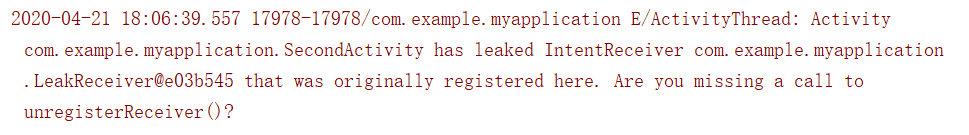
\includegraphics[width=0.9\textwidth]{broadcast_leak.png} % requires the graphicx package
	\caption{没有回收接收器将会导致异常以及泄露}
	\label{fig:broadcast_leak}
\end{figure}

\subsection{广播接收器的注册方式}
\begin{listing}[htbp]
	\centering
	\caption{广播接收器的注册方式}
	\begin{minted}[encoding=utf8,
	frame=single,
	framesep = 1em,
	numbers=left, 
	breaklines=true, 
	tabsize=4,
	showtabs = false,
	xleftmargin=2em,xrightmargin=2em,
	fontsize=\footnotesize]{XML}
<manifest 
	xmlns:android="http://schemas.android.com/apk/res/android"
	xmlns:dist="http://schemas.android.com/apk/distribution"
	package="com.example.myapplication">
	<dist:module dist:instant="true" />
	<application ...>
		...
		<receiver
			android:name = ".Receiver1">
			<intent-filter>
				<action android:name = "act1" />
			</intent-filter>
		</receiver>
		<receiver
			android:name = ".Receiver2"
			android:exported = "false"
			android:enabled = "true">
			<intent-filter>
				<category android:name = "cat1" />
				<action android:name = "act2" />
			</intent-filter>
		</receiver>
	</application>
</manifest>
	\end{minted}
	\label{declaration:receiver}
\end{listing}

一般而言,清单声明的广播接收器(见\ref{declaration:receiver in manifest})需要在\textbf{AndroidManifest.xml}文件中添加\textbf{<receiver>}标签(参考\textbf{Listing.\textcolor{red}{\ref{declaration:receiver}}}),在\textbf{<intent-filter>}子标签中可以指定订阅的广播内容等,也可以通过设置\textbf{"android:exported"}属性来指定该广播是否将被导出。而上下文注册的广播接收器(见\ref{declaration:receiver in context})则不需要进行前文的操作。
\subsection{广播接收器的内存泄漏}
广播接收器的内存泄漏原理类似与服务内存泄漏\ref{service_leak}。但是由广播接收器引起的内存泄漏往往比服务更为严重,因为广播接收器被系统认为只进行不耗时的操作(如果超过10s未从\textbf{onReceive()}方法中返回,将抛出\textbf{ANR(Application Not Response)异常}),因此通常广播接收器在接到广播后,很有可能会启动其他的\textbf{Service}进行后续的耗时操作,进而可能会导致一连串的内存泄漏。

例如图中(见\textbf{Listing.\textcolor{red}{\ref{leaked example:receiver}}})所示的广播接收器,不仅本身会导致内存泄漏,而且还会启动一个会导致内存泄漏的服务(见\textbf{Listing.\textcolor{red}{\ref{leaked example:service}}}),因此后果将会更加严重。
\begin{listing}[htbp]
	\centering
	\caption{广播接收器的内存泄漏}
	\begin{minted}[encoding=utf8,
	frame=single,
	framesep = 1em,
	numbers=left, 
	breaklines=true, 
	tabsize=4,
	showtabs = false,
	xleftmargin=2em,xrightmargin=2em,
	fontsize=\footnotesize]{java}
public class LeakReceiver extends BroadcastReceiver {
	private final String TAG = "LeakReceiver";
	private final int ID = new Random().nextInt();
	@Override
	public void onReceive(Context context, Intent intent) {
		...
		context.startService(new Intent(context,LeakService.class));
		new Timer().scheduleAtFixedRate(()->{
			Log.i(TAG,LeakReceiver.this.ID + " is running!");
		}, 1000L, 3000L);
	}
}
	\end{minted}
	\label{leaked example:receiver}
\end{listing}

\section{小结}

本章首先介绍了安卓系统的发展历史,以及安卓应用的四大主要组件,意在说明不可见控件在安卓应用中的重要作用。

接下来重点说明了两类不可见组件(服务和广播)的注册、启动方式,及其生命周期,然后举例说明了组件产生内存泄漏的原因,以及内存泄漏将会导致的严重后果。为后文的检测提供依据。